 \documentclass{report}
 
\usepackage[utf8]{inputenc} 
\usepackage[T1]{fontenc}      
\usepackage[top=2.0cm, bottom=3cm, left=3.0cm, right=3.0cm]{geometry}
\usepackage{graphicx}
\usepackage{wrapfig}
\usepackage{amsmath,esint }
\usepackage{amssymb}
\usepackage{esvect}
\graphicspath{{figures/}{../figures}}

\newcommand*\dif{\mathop{}\!\mathrm{d}}
\newcommand*\diver{\mathop{}\!\mathrm{div}}
\newcommand*\grad{\mathop{}\!\mathrm{grad}}

\begin{document}

\section*{Volatiles sur une ligne à haute tension $\bullet\circ\circ$}

L'étourneau sansonnet est une espèce d'oiseau sociale, se déplaçant par groupe de centaines, voire de milliers d'individus. On peut les apercevoir suspendus sur des lignes électriques avant leur envol. Pour notre étude, on peut modéliser l'étourneau comme une sphère de rayon $R=10$cm parfaitement conductrice (les tissus biologiques étant de bons conducteurs électriques). 

\begin{itemize}

	\item[$\bigvee$] Un étourneau se pose sur une ligne électrique au potentiel $V=50$kV. Quelle charge $Q$ va t-il porter à ce potentiel ? \textit{NB} : Les lignes électriques n'ont pas de revêtement isolant.
	
	\item[$\bigvee$] En réalité, la tension est alternative, à la fréquence $f=50$ Hz. Sachant que l'intensité létale est d'environ 10mA, l'étourneau prend-il un risque à se poser dessus ?
	
	\item[$\bigvee$] Un nuée de 1000 étourneaux se pose instantanément sur cette ligne électrique. Quelle va être la diminution de puissance électrique (temporaire) au bout de la ligne ?

\end{itemize} 

\newpage

\section*{\textit{Correction Volatiles sur une ligne à haute tension}}

\begin{itemize}

	\item[$\bigvee$] L'oiseau est une sphère de rayon $R$ portée au potentiel $V$ par rapport au sol, supposé très loin. Le potentiel est alors (à redémontrer par l'élève) :
	\begin{align*}
		V=\frac{Q}{4\pi\varepsilon_0 R}
	\end{align*}
	Il se charge donc d'une charge $Q=V\times 4\pi\varepsilon_0R=5,6\times10^{-7}$C.
	
	\item[$\bigvee$] Le courant étant alternatif, l'oiseau se charge et se décharge de $Q$ 50 fois par seconde. Il est donc parcouru par une intensité au minimum de $I=Qf=27\mu$A. On est loin du poulet rôti...
	
	\item[$\bigvee$] Lorsque les oiseaux se posent, il y a instantément une déviation de courant qui s'opèrent vers eux pour les monter à la charge $Q$. Il y a donc $N$ fois le courant $I$ qui est dévié le temps d'une période de charge, soit 27mA. Les ampérages circulant dans les lignes étant typiquement de l'ordre de l'ampère, on est loin d'avoir des problèmes liés à ces volatiles.

\end{itemize} 

\newpage		

\section*{Champ dans une cavité $\bullet\bullet\circ$}

Une boule de centre $O_1$ et de rayon $a$ portant une charge volumique uniforme $\rho$ possède une cavité sphérique de centre $O_2$ de rayon $b$ vide de charges.

\begin{figure}[h!]
\centering
		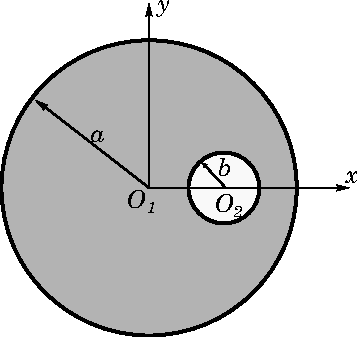
\includegraphics[scale=0.7]{em_cavite.pdf}
\end{figure}

\begin{itemize}

	\item[$\odot$] Déterminer le champ électrique $\vec{E}$ et le potentiel $V$ associé dans la cavité.

\end{itemize}

Désormais, on suppose que la boule est constituée d'un matériau conducteur. On suppose que pour ces matériaux, les charges ne se répartissent pas en volume ($\rho=0$) mais uniquement sur les surfaces ($\sigma\neq0$) de sorte que le champ électrique est toujours nul dans un tel matériau. 

\begin{itemize}

	\item[$\odot$] Montrer que le champ électrique est nul dans la cavité. Peut-il y avoir des charges sur la surface interne entre la cavité et le matériau conducteur ?
	
\end{itemize}

On place désormais une charge $+q$ au centre de la cavité, en $O_2$. 

\begin{figure}[h!]
\centering
		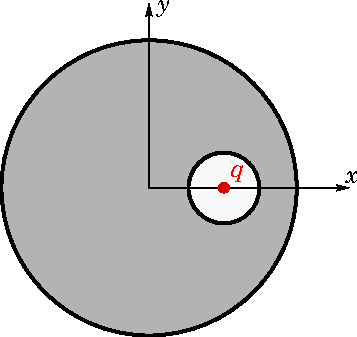
\includegraphics[scale=0.7]{em_cavite2.pdf}
\end{figure}

\begin{itemize}
	
	\item[$\odot$] Montrer qu'une charge surfacique $\sigma$ se répartit uniformément sur la surface interne et l'exprimer en fonction de $b$ et $q$.
	
	\item[$\odot$] La charge totale du matériau conducteur étant nulle, montrer qu'une charge surfacique $\sigma'$ se répartit sur la surface externe. Quel est le champ électrique à l'extérieur (pour $r>a$) ? 

\end{itemize}

\textit{NB} : On rappelle qu'à l'interface d'une surface chargée $\sigma$ entre 2 milieu 1 et 2, la composante normale du champ électrique n'est pas continue : $\vec{E}_{N,2}-\vec{E}_{N,1}=\frac{\sigma}{\varepsilon_0}\vec{n}_{1\rightarrow2}$, où $\vec{n}_{1\rightarrow2}$ est le vecteur normale entre l'interface 1 et 2.



\newpage

\section*{Champ créé par deux sphères $\bullet\circ\circ$}

On considère deux sphères de rayon $R$, situées respectivement en $O_1$ et en $O_2$, de telle sorte que $\vv{O_1O_2}=d\vec{e}_x$, avec $d\gg R$. La sphère située en $O_1$ porte une charge $+Q_1$, celle en $O_2$ porte une charge $Q_2$, charges que l'on supposera uniformément réparties. 

\begin{itemize}

	\item[$\oplus$] Quel est le champ électrique $\vec{E}_1$ créé par la sphère 1 ? Quel est le champ créé par les deux sphères ? On admettra que le champ électrique des sphères est équivalent à celui d'une particule ponctuelle portant la même charge.
	
	\item[$\oplus$] En déduire le potentiel électrique $V_1(\vec{r})$ créé par la sphère 1, puis le potentiel total $V(\vec{r})$ créé par les deux sphères. Le potentiel est supposé nul à l'infini. On exprimera le résultat en coordonnées cartésiennes.
	
	\item[$\oplus$] Tracer sur un schéma les lignes de champs et les équipotentielles. 
	
	\item[$\oplus$] Une charge $+e$ est évacuée de la surface de la sphère 1, au niveau de l'axe $\vv{O_1O_2}$, avec une vitesse initiale $\vec{v}=v_0\vec{e}_x$. A quelle vitesse arrive t-elle sur la sphère 2 ? On simplifiera le résultat en prenant $Q_1=-Q_2=+Q$.
	
	\item[$\oplus$] Que se passe t-il si la sphère 2 porte une charge désormais $Q_2=+Q$ ? Quelle est la nature du mouvement ?

\end{itemize}

\newpage

\section*{Champ créé par deux fils infinis $\bullet\circ\circ$}

On considère deux fils d'axe directeur $\vec{e}_z$, de rayon $R$ et très long $L\gg R$. Ils situés respectivement en $O_1$ et en $O_2$, de telle sorte que $\vv{O_1O_2}=d\vec{e}_x$, avec $d\gg R$. Le fil situé en $O_1$ porte une charge $Q_1$, celui en $O_2$ porte une charge $Q_2$, charges que l'on supposera uniformément réparties. 

\begin{itemize}

	\item[$\oplus$] Pourquoi peut-on parler de densité linéique de charge $\lambda_1$ (resp. $\lambda_2$) du fil 1 (resp. du fil 2) ? Les calculer.

\end{itemize}

On admet que le champ électrique créé par un fil infini de charge linéique $\lambda$ d'axe directeur $\vec{e}_z$, passant par l'origine $O$, s'écrit en coordonnées cylindriques :
\begin{align*}
	\vec{E}=\frac{\lambda}{2\pi\varepsilon_0 r}\vec{e}_r
\end{align*}

\begin{itemize}

	\item[$\oplus$] En déduire le potentiel électrique $V_1$ créé par le fil 1, puis le potentiel total $V(\vec{r})$ créé par les deux fils. On écrira le résultat en coordonnées cartésiennes.
	
	\item[$\oplus$] Tracer sur un schéma les lignes de champs et les équipotentielles. 
	
	\item[$\oplus$] Une charge $+e$ est évacuée du fil 1, au niveau de l'axe $\vv{O_1O_2}$, avec une vitesse initiale $\vec{v}=v_0\vec{e}_x$. A quelle vitesse arrive t-elle sur le fil 2 ? On simplifiera le résultat en prenant $Q_1=-Q_2=+Q$.
	
	\item[$\oplus$] Que se passe t-il si le fil 2 porte une charge désormais $Q_2=+Q$ ? Quelle est la nature du mouvement ? 

\end{itemize}

\newpage

\section*{Champ créé par deux plans infinis $\bullet\circ\circ$}

On considère deux plans "épais" de vecteur normal $\vec{e}_x$, d'épaisseur $e$, de surface $S$ très grande : $S\gg e$. Ils situés respectivement en $O_1$ et en $O_2$, de telle sorte que $\vv{O_1O_2}=d\vec{e}_x$. Le plan situé en $O_1$ porte une charge $+Q_1$, celui en $O_2$ porte une charge $Q_2$, charges que l'on supposera uniformément réparties. 

\begin{itemize}

	\item[$\oplus$] Pourquoi peut-on parler de densité surfacique de charge $\sigma_1$ (resp. $\sigma_2$) du plan 1 (resp. du plan 2) ? Les calculer.

\end{itemize}

On admet que le champ électrique créé par un plan infini de charge surfacique $\sigma$ de vecteur normal $\vec{e}_x$, passant par l'origine $O$, s'écrit en coordonnées carthésiennes :
\begin{align*}
	\vec{E}=\frac{\sigma}{2\varepsilon_0}\mathrm{sign}(x)\vec{e}_x
\end{align*}

\begin{itemize}

	\item[$\oplus$] En déduire le potentiel électrique $V_1$ créé par le plan 1, puis le potentiel total $V(x)$ créé par les deux plans.
	
	\item[$\oplus$] Tracer sur un schéma les lignes de champs et les équipotentielles. 
	
	\item[$\oplus$] Une charge $+e$ est évacuée de la surface du plan 1, au niveau de l'axe $\vv{O_1O_2}$, avec une vitesse initiale $\vec{v}=v_0\vec{e}_x$. A quelle vitesse arrive t-elle sur le plan 2 ? On simplifiera le résultat en prenant $Q_1=-Q_2=+Q$.
	
	\item[$\oplus$] Que se passe t-il si le plan 2 porte une charge désormais $Q_2=+Q$ ? Quelle est la nature du mouvement ? 

\end{itemize}

\newpage

\section*{Capacité créée par deux fils infinis parallèles $\bullet\bullet\circ$}

On considère deux cylindres infiniment longs de rayon $a$, notés 1 et 2, tous deux d'axe directeur $Oz$ et passant respectivement par $x=-d/2$ et $x=+d/2$, avec $d>a$. Ils sont uniformément chargés en volume, avec $\rho_1=-\rho_2=\rho$.

\begin{itemize}

	\item[$\oplus$] En déduire le potentiel électrique $V_1$ créé par le cylindre 1, puis le potentiel total $V(\vec{r})$ créé par les deux fils. On écrira le résultat en coordonnées cartésiennes.
	
	\item[$\oplus$] Tracer sur un schéma les lignes de champs et les équipotentielles. 
	
	\item[$\oplus$] En déduire la tension électrique $U$ entre la surface des deux cylindres, en supposant qu'elle sont elles-mêmes des surfaces équipotentielles.
	
	\item[$\oplus$] La capacité linéique $\Gamma$ est la capacité équivalent $C$ d'un condesateur d'un tronçon de longueur $L$ selon $z$ de ce dispositif, divisé par $L$, soit $C=\Gamma/L$. Déterminer $\Gamma$.

\end{itemize}

\newpage

\section*{Champ créé par deux plans infinis $\bullet\bullet\circ$}

On considère deux plans "épais" de vecteur normal $\vec{e}_x$, d'épaisseur $e$, de surface $S=L_y\times L_z$ très grande : $L_y,L_z\gg e$. Ils situés respectivement en $O_1=O$ (où $O$ est l'origine du repère de coordonnées carthésiennes) et en $O_2$, de telle sorte que $\vv{O_1O_2}=d\vec{e}_x$. Le plan situé en $O_1$ porte une charge $Q_1$, celui en $O_2$ porte une charge $Q_2$, charges que l'on supposera uniformément réparties dans le volume. 

\begin{itemize}

	\item[$\oplus$] Quelle sont les charges volumiques associées aux plan 1 et 2, notées $\rho_1$ et $\rho_2$ ? En déduire le champ électrique $\vec{E}$ créé dans tout l'espace.

	\item[$\oplus$] En déduire le potentiel total $V(x)$ créé par les deux plans.
	
	\item[$\oplus$] Tracer sur un schéma les lignes de champs et les équipotentielles. 
	
	\item[$\oplus$] On suppose que $Q_1=-Q_2=Q$. Une charge $+e$ arrive depuis les $x$ décroissants avec une vitesse initiale $\vec{v}=v_0\vec{e}_x$. On suppose qu'elle peut traverser les plans chargés sans autre interation que celle électromagnétique. A quelle condition sur $v_0$ arrive t-elle à passer outre le second plan ? 
	
	\item[$\oplus$] On retire maintenant le plan 2 ($Q_2=0$) et on suppose que le plan 1 est infiniment fin $e\longrightarrow0$, toujours chargé positiviment. Après avoir introduit la densité de charge surfacique $\sigma_1$, calculer le champ électrique résultant puis en déduire le mouvement d'une particule $-e$ autour de l'axe $Ox$.

\end{itemize}

\newpage

\section*{Interaction entre un plan chargé et une charge $-q$ $\bullet\circ\circ$}

On considère une nappe de charge, comprise entre $x=-a/2$ et $x=a/2$, et infiniment étendue selon les axes $y$ et $z$, avec une densité volumique de charge $\rho>0$.

\begin{itemize}

	%\item[$\heartsuit$] A l'aide des invariances et des symétries, montrer que $\vec{E}=E(x)\vec{e}_x$.

	\item[$\heartsuit$] Déterminer le champ électrique $\vec{E}$ et le potentiel $V$ en tout point de l'espace.
	
	\item[$\heartsuit$] Une charge ponctuelle $-q$ peut se mouvoir librement selon l'axe $Ox$. Déterminer la nature de son mouvement en supposant que sa vitesse est nulle en $x=b<a_2$.
	
	\item[$\heartsuit$] On suppose désormais que la nappe est infiniment fine, c'est-à-dire que $a\longrightarrow0$, mais que $\rho\longrightarrow\infty$ de sorte que la charge contenue dans un volume $V$ passant par le plan reste finie. Introduire une densité surfacique de charge $\sigma$, puis donner les expressions de $\vec{E}$ et de $V$.
	
	\item[$\heartsuit$] Déterminer le mouvement de la charge $-q$ dans ce cas-là. 
	
\end{itemize}

\newpage

\section*{Sphère uniformément chargée}
Soit une sphère de rayon $R$, de centre $O$ et de densité surfacique de charge uniforme $\sigma$.

\begin{itemize}
\item Donner les symétries et les invariances de la distribution de charges, et en déduire l'orientation et la dépendance spatiale du champ électrostatique en tout point de l'espace.
\item Appliquer le théorème de Gauss afin de déterminer le champ électrostatique en un point $M$ situé à une distance $r=OM>R$. En déduire le potentiel électrostatique en $M$ (on choisira le potentiel nul à l'infini).
\item Déterminer le champ électrostatique en un point $M$ situé à une distance $r=OM<R$. En déduire le potentiel électrostatique en $M$.
\item Représenter $E(r)$ et $V(r)$ sur un graphique.
\item La Terre a un rayon $R=$6400 km et porte à sa surface une densité surfacique de charge uniforme $\sigma=-10^{-9}$ C$\cdot$m$^{-2}$.

Quelle est la différence de potentiel entre la surface de la Terre et un point situé à 2 m au-dessus ? On donne $\dfrac{1}{4\pi\varepsilon_0}=9\cdot 10^9$ SI.

Pourquoi un homme ne ressent-il pas cette différence de potentiel ? % corps humain conducteur donc au potentiel de la Terre en tout point.
\end{itemize}

\newpage

\section*{Potentiel de Yukawa $\bullet\bullet\circ$}

\`{A} une distance $r$ d'un point $O$, le potentiel électrostatique créé par une certaine distribution de charges a pour expression :
$$
V(r)=\frac{e}{4\pi \epsilon_0r}\exp\left( -\frac{r}{a_0}\right) 
$$
où $a_0$ est une longueur caractéristique et $e$ la charge élémentaire.

\begin{enumerate}
\item Calculer le champ $\vec{E}$ à une distance $r$ du point $O$ et le flux $\Phi$ de ce champ à travers une sphère de rayon $r$ et de centre $O$. En déduire la charge intérieure à cette sphère $Q_{\mathrm{int}}$. 
\item Que deviennent ces expressions quand $r\rightarrow 0$ ? Interpréter. Idem quand $r\rightarrow +\infty$.\\ Quel système le potentiel de Yukawa peut modéliser ?
\item Calculer la densité volumique de charge $\rho$ à une distance $r$ de $O$. On décomposera $Q_{\mathrm{int}}$ en une charge ponctuelle en $O$ et une charge volumique diffuse pour $r>0$. Calculer $q'$ somme des charges négatives contenues dans la sphère de centre $O$ et de rayon $r$.
\item \'{E}tudier la variation, en fonction de $r$, de la grandeur $z=4\pi r^2\rho$ appelée \textit{densité radiale de charge}. Donner une interprétation de la longueur caractéristique $a_0$.
\end{enumerate}

\newpage

\section*{Effet d'une charge d'espace $\bullet\bullet\circ$}

Un faisceau d'ions or $Au^+$ de charge $e$ et de masse $m$ créé dans la zone $z<0$ pénètre à une vitesse négligeable dans la zone $z>0$ vide, à travers une plaque $P$ percée en $O$ et portée au potentiel nul dans le plan $xOy$. Une autre plaque, $P'$, parallèle à $P$, placée en $z=l>0$ et percée au point $I(0,l)$ est portée au pontentiel $V_0<0$. 

Toutes les propriétés du système sont invariantes par translation dans le plan $xOy$ et on considère uniquement les mouvements de charges dans la direction $Oz$ en régime permanent. On considère de plus que le faisceau d'ions est supposé avoir une section $S$ uniforme et que le champ électrique  àl'intérieur est sous la forme $\vec{E}=E(z)\vec{e}_z$.

\begin{figure}[h!]
\centering
		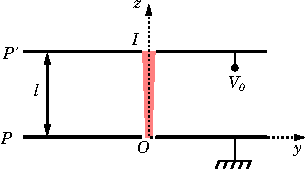
\includegraphics[scale=1.3]{em4.pdf}
\end{figure}

Pour des jets d'ions intenses, il faut tenir compte des effets d'influences électrostatique entre les ions présents entre les plaques, où réside une charge d'espace. On appelle respectivement $\rho(z)$, $V(z)$, et $\nu(z)$ la densité volumique de charge, le potentiel électrostatique et la valeur du champ des vitesses des ions à la distance $z$ du plan $xOy$. 

\begin{itemize}

	\item[$\blacktriangle$] Rappeler l'expression de la conservation de la charge. Pourquoi le produit $\rho(z)\nu(z)$ est il indépendant de $z$ en régime permanent ? 
	
	\item[$\blacktriangle$] En écrivant le théorème de Gauss sur un volume du faisceau d'ions compris entre $z$ et $z+dz$, montrer :
	\begin{align*}
		\frac{\partial^2 V}{\partial z^2}=-\frac{\rho(z)}{\varepsilon_0}
	\end{align*}
	
	\item[$\blacktriangle$] Ecrire le théorème de l'énergie cinétique pour obtenir une autre éqution sur $V(z)$, $\rho(z)$ et $\nu(z)$. 
	
	\item[$\blacktriangle$] En déduire l'équation différentielle satisfaite par $V(z)$. 
	
	\item[$\blacktriangle$] Résoudre cette équation différentielle, et en déduire la relation de Child-Langmuir donnant la densité de courant $j_z$ :
	\begin{align*}
		j_z =\frac{4}{9}\varepsilon_0\sqrt{\frac{2e}{m}}\frac{(-V_0)^{3/2}}{l^2}
\end{align*}		
On rappelle que la densité de courant $\vec{j}$ est définie par $\vec{j}=\rho\vec{\nu}$.
	
\end{itemize}

\newpage

\section*{Étude d'un colloïde $\bullet\bullet\circ$}

Un colloïde est une solution constituée d'un solvant (de l'eau et des ions) et de particules solides, \textit{dites de colloïde}, en suspension dont la taille peut varier de 10 à 100nm et qui se chargent dans le solvant. Par exemple, du lait ou de la terre dans l'eau sont des solutions colloïdales.

Lorsqu'on augmente la concentration ionique de la solution (en ajoutant du sel par exemple) on observe la sédimentation de la solution colloïdale (les particules de colloïde "tombent" au fond du récipient) : ce phénomène est appelé \textit{floculation} et on cherche à le décrire ici.

Pour décrire le phénomène, on supposera que la solution colloïdale est composée de :
\begin{itemize}
	\item[-] des particules de colloïdes, de rayon $r_0$, portant une charge $Q$ sur leur surface. Ils sont supposés assez dilués pour considérer que le potentiel autour d'une particule colloïdale n'est créée que par elle-même et les ions du milieu ;
	\item[-] les ions contenus dans l'eau à la concentration $N_0$, supposés ponctuels, portant une charge $\pm e$. On supposera que la concentration en cations est égale à celle en anions. Les ions (cations + ou anions -), quand il sont soumis à un potentiel extérieur $V$, se répartissent en moyenne selon la loi de Boltzmann :
\begin{align*}
	\frac{N_{\pm}(r)}{N_0}=\exp\left(-\frac{\pm eV(r)}{k_BT} \right) 
\end{align*}
\end{itemize}
La permitivité du milieu est $\varepsilon=\varepsilon_r\varepsilon_0$ avec $\varepsilon_r=80$. On s'intéresse à une particule de colloïde en suspension dans la solution, entourée d'ions.

%Lorsqu'on augmente significativement la concentration $N_0$ de la solution ionique, on observe que la suspension colloïdale sédimente très rapidement. On cherche à comprendre ce phénomène appelé \textit{floculation}. Pour cela, on s'intéresse à une particule de colloïde en suspension dans la solution, entourée des ions. 

\begin{itemize}

	\item[$\heartsuit$] S'il n'y avait pas d'ions en solution, quel serait le potentiel $V(r)$ autour de la particule de colloïde ? Décrire brièvement comment se répartiraient alors des ions s'ils étaient soumis à ce potentiel.

\end{itemize}

En réalité, la présence de ces ions modifie le potentiel $V$ autour de la particule, qui modifie à son tour la présence d'ions (à travers la densité de charge $\rho$). On souhaite donc trouver deux équations sur $V(r)$ et $\rho(r)$ pour les déterminer. 

\begin{itemize}

	\item[$\heartsuit$] Établir la densité volumique de charge entourant une particule de colloïde. Que devient cette expression si $eV\ll k_BT$ ?
	
	\item[$\heartsuit$] En appliquant le théorème de Gauss, une fois sur une sphère de rayon $r$ autour de la particule, puis une seconde fois en $r+dr$, montrer que : 
	\begin{align*}
		\frac{1}{r^2}\frac{\dif}{\dif r}\left( r^2\frac{\dif V}{\dif r}\right) +\frac{\rho}{\epsilon}=0
	\end{align*}

	\item[$\heartsuit$] Résoudre l'équation différentielle en posant $U(r)=rV(r)$, et retrouver l'expression de $V(r)$, en fonction de $r$, une longueur caractéristique $\lambda$ et une constante d'intégration qu'on ne cherchera pas à définir. Donner un ordre de grandeur de $\lambda$ à température ambiante dans de l'eau pure.
	
	\item[$\heartsuit$] Écrire l'expression du champ électromagnétique. En déduire la constante d'intégration, et l'expression de $V(r)$. 
	
	\item[$\heartsuit$] Quelle est l'expression de la densité de charge $\rho$ ? Justifier l'appellation d'\textit{écrantage}.
	
	\item[$\heartsuit$] Quelle est la force $F(d)$ qui s'exerce entre deux particules de colloïde éloignées d'une distance $d$ ? Comparer cette force dans le cas d'une eau pure et celle d'une électrolyte de concentration $N_0=10^{-7}$mol/L. Pourquoi parle t-on de coagulation ?

\end{itemize} 

\newpage

\section*{Condensateur Terre-ionosphère $\bullet\circ\circ$}

On représente l'ensemble Terre-ionosphère comme un volumineux condensateur sphérique. La Terre, de rayon $R$, se comporte comme un conducteur parfait de potentiel nul et porte une charge négative $-Q$, uniformément répartie sur sa surface, tandis que la ionosphère est représentée par une surface équipotentielle sphérique de rayon $R+z_0$, de potentiel $V$ possède une charge totale $+Q$. On suppose que la permittivité de l'atmosphère est celle du vide, soit $\varepsilon_0$. 

\begin{figure}[h!]
\centering
		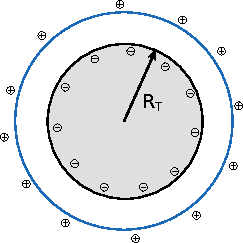
\includegraphics[scale=1]{em3.pdf}
\end{figure}

\begin{itemize}

	\item[$\clubsuit$] Lorsqu'un conducteur parfait est suoumis à un champ électrique extérieur, le champ électrique est nul à l'intérieur de ce conducteur et il se charge en surface. Rappeler pourquoi.
	
	\item[$\clubsuit$] Déterminer le champ électrique $\vec{E}(r)$.
		
	\item[$\clubsuit$] En déduire la capacité $C$ du système Terre-ionosphère.
	
	\item[$\clubsuit$] Des mesures ont permis de déterminer le potentiel de l'ionosphère à l'altitude $z_0=60$km à environ 360kV. Justifier que le système se comporte comme un condensateur plan. Quel est la valeur de la capacité $C$ et l'énergie électrostatique du système $W_{el}$, ainsi que la valeur du champ électrique au niveau du sol.
	
	\item[$\clubsuit$] Donner la valeur de la densité de charge $\sigma$ à la surface de la Terre. Quelle est la charge totale $-Q$ ?
	
	\item[$\clubsuit$] Lors d'un orage, les mouvements convectifs de l'air font passer la tension augmentent fortement la tension entre le sol et le bas des nuages. Les éclairs apparaissent lorsque le champ électrique dépasse un seuil, appelé \textit{champ disruptif} : l'air s'ionise et devient conducteur. Sachant que pour un air humide, ce champ disruptif est de $E_{dis.}\simeq10^{5}$V.m$^{-1}$. A quelle tension $V_1$ observe t-on l'apparition des éclairs ?
	
	
	\textit{Données} : Rayon de la Terre, $R_T=6370$km. Permittivité du vide, $\varepsilon=8,85\cdot10^{-12}$F.m$^{-1}$.
	
\end{itemize}

\newpage

\section*{Condensateur sphère-plan $\bullet\bullet\bullet$}

On considère un conducteur parfait plan, situé en $z=0$ et une particule ponctuelle, elle aussi parfaitement conductrice, dont le centre est situé en $(x=0, y=0, z=d)$. La sphère est portée au potentiel $V$ tandis que le plan est relié à la masse, c'est-à-dire au potentiel nul. Le but de l'exercice est de déterminer la capacité entre le plan et la sphère.

\begin{itemize}

	\item[$\circ$] 

\end{itemize}

\newpage

\end{document}
